\documentclass[tikz,border=10pt]{standalone}

\begin{document}
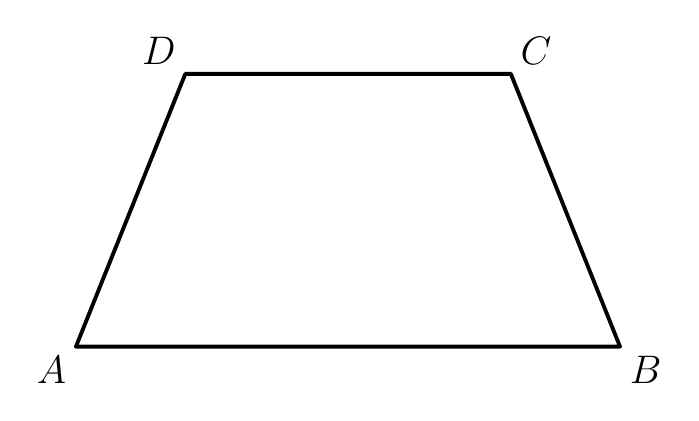
\begin{tikzpicture}
\coordinate (A) at (-3.483,-1.723);
\coordinate (B) at (3.427,-1.723);
\coordinate (C) at (2.041,1.741);
\coordinate (D) at (-2.094,1.741);

  
  
  \draw[line width=1.4pt, line join=round] (A) -- (B) -- (C) -- (D) -- cycle;
  
  \node[below left]  at (A) {\fontsize{14.5}{17.4}\selectfont $A$};
  \node[below right] at (B) {\fontsize{14.5}{17.4}\selectfont $B$};
  \node[above right] at (C) {\fontsize{14.5}{17.4}\selectfont $C$};
  \node[above left]  at (D) {\fontsize{14.5}{17.4}\selectfont $D$};
\end{tikzpicture}
\end{document}